\section{Differencing issues} \label{sec:risk_diff}

A differencing problem can occur when releasing data for two or more different geographical areas. The difference between the two areas can locally lead to disclosure of confidential information, especially small population counts. The difference can be made between two nested areas\footnote{
    For example, at the European level, the NUTS levels are such nested sets of areas: NUTS3 $\subseteq$ NUTS2 $\subseteq$ NUTS1.} 
as in tabular data, but the problem is more acute for geo-referenced data released on several overlapping geographical areas. Nowadays, it is common for National Statistical Institutes (NSI) to seek to publish census data not only over many administrative areas but also over grid cells. To handle these kinds of cases can be very difficult, especially when a suppressive method is used.

As the differencing by nested geographical areas is not so different from the differencing by any hierarchical variable in tabular data, one can read \citet[4.3.1]{HundepoolEtAl2024} to learn how to deal with it. In the following, only overlapping areas are considered.

The differencing issue is presented in \citet[5.2]{HundepoolEtAl2024} and \cite{BuronFontaine2018}. \cite{Duke-Williams_Rees_1998} details how the issue is tackled for the release of UK census data in the simplest case of overlapping. \cite{Costemalle_2018}  and \cite{Costemalle_2019} present a way to detect all differencing issues when two non-nested geographical areas are released at the same time. This method is implemented in an R package called \texttt{diffman} \citep{diffman}. The presentation is based on the way \cite{Costemalle_2019} detects differencing issues.

\subsection{A first example}

\begin{figure}[H]
\centering
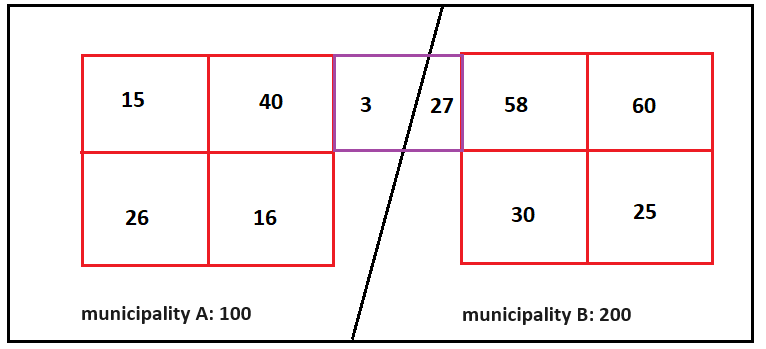
\includegraphics[width=\linewidth]{figures/Differencing_issues/protection_process_0_en.png}
\caption{A first example of geographical differencing.}
\label{fig:cas_complex_12}
\end{figure}

Figure~\ref{fig:cas_complex_12} represents two municipalities and all the  $1$~km $\times$ $1$~km grid tiles intersecting at least one of the municipalities. Municipality $A$ has $100$~households, municipality $B$ has $200$. The number of households in each of the tiles is also disseminated. Let us consider that an information is considered confidential if it concerns fewer than $4$ households. Releasing household counts over both geographical areas generates no direct confidentiality issue, all counts being greater than $4$.

As two sets are released, the difference can be processed:

\begin{equation}
    \begin{split}
    A &= 100 = 15 + 40 + 26 + 16 + A^{\cap B} \\
    B &= 200 = 58 + 60 + 30 + 25 + B^{\cap A} \\
    %30 &= x + y , no need for this equation
    \end{split}
    \label{eq:diff_interne}
\end{equation}

where:

\begin{itemize}
\item \(A^{\cap B}\) denotes the number of households in the tile intersecting A and B residing in municipality A.
\item \(B^{\cap A} \) denotes the number of households in that tile residing in municipality B. 
\end{itemize}

We then obtain the following indirectly released information :

\begin{equation}
    \begin{split}
    A^{\cap B} &= 3 \\
    B^{\cap A} &= 27 
    \end{split}
    \label{eq:diff_interne2}
\end{equation}

In this specific case, an attacker can easily retrieve a confidential information by differencing the two areas.


As \cite{Costemalle_2019} introduced a systematic detection of differencing issues, the following subsections will be based on the way the problem is described there.

\subsection{Internal and external differencings}

The \textit{internal region} of the municipality $A$ is composed by all the tiles which are fully included in $A$ \citep{Costemalle_2019}. If $A_{intern}$ and $B_{intern}$ denote the counts associated with internal regions of $A$ and $B$ respectively, we get from the figure~\ref{fig:cas_complex_12}:

\begin{equation}
    \begin{split}
    A_{intern} &= 15+40+26+16 = 97 \\
    B_{intern} &= 58+60+30+25 = 173 
    \end{split}
    \label{eq:internal_regions}
\end{equation}

An \textit{internal differencing} is then the difference between an area and its internal region, as shown in equation~(\ref{eq:diff_internal}) for $A$ and $B$ municipalities.

\begin{equation}
    \begin{split}
    A - A_{intern} &= 100 - 97 = 3 \\
    B - B_{intern} &= 200 - 173 = 27 
    \end{split}
    \label{eq:diff_internal}
\end{equation}

Symmetrically, the \textit{external region} of the municipality $A$ is composed by all the tiles which are fully included \emph{or} partially included in $A$ \citep{Costemalle_2019}. If $A_{extern}$ and $B_{extern}$ denote the external regions of $A$ and $B$ respectively, we get from the figure~\ref{fig:cas_complex_12}:

\begin{equation}
    \begin{split}
    A_{extern} &= 15+40+26+16+30 = 127 \\
    B_{extern} &= 58+60+30+25+30 = 203 
    \end{split}
    \label{eq:external_regions}
\end{equation}

An \textit{external differencing} is then the difference between an area and its external region, as shown in the equation~(\ref{eq:diff_external}) for $A$ and $B$ municipalities.

\begin{equation}
    \begin{split}
    A_{extern} - A &= 127 - 100 = 27 \\
    B_{extern} - B &= 203 - 200 = 3 
    \end{split}
    \label{eq:diff_external}
\end{equation}

Hence, a differencing issue, for a given region $A$, occurs when the internal or external difference is under the threshold but greater than $0$.

\subsection{Complexity}

\begin{figure}[H]
    \centering
    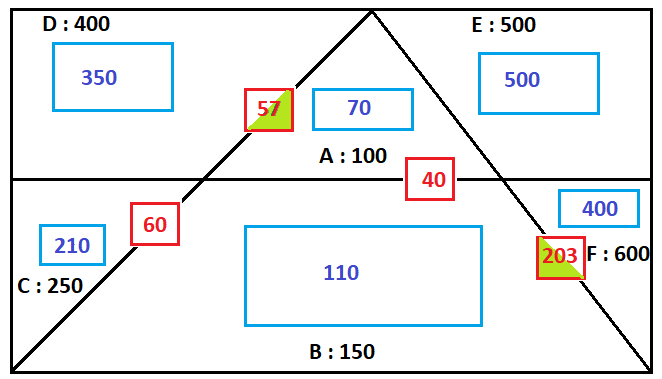
\includegraphics[width=0.8\linewidth]{figures/Differencing_issues/schema_intermediaire.png}
    \caption{A more complex differencing case.}
    \vspace{0.1cm}
    \raggedright \textit{Reading Note: In black the population of municipalities; in blue the number of households in tiles internal to municipalities; in red the number of households in tiles intersecting 2 municipalities.}
    \label{fig:schema_inter}
\end{figure}

Figure~\ref{fig:schema_inter} shows a case that is a little bit more complex, with six municipalities ($A, \dots , F$) whose household counts are displayed in black. The internal counts of each municipality are represented by the blue squares and the overlapping tiles by the red squares. 

Internal and external differencing can be performed for each municipality. For example, applying external differencing to the municipality $F$, we get $F_{extern} - F = 603 - 600 = 3$, which discloses a confidential information according to the chosen threshold. This external differencing is the counterpart of the internal differencing of the area composed by $A$, $B$, $C$ and $D$: $ABCD - ABCD_{intern} = 100 + 150 + 250 + 400) - (70 + 40 + 110 + 60 + 210 + 350 + 57) = 900 - 897 = 3$. Hence, possibly involving many areas at once, differencing problems can be hard to detect with real geographical areas.


\subsection{Method to detect differencing problems implemented in the \texttt{diffman} package} \label{sec:risk_diff_diffman}

When releasing data over administrative areas and $1$~km grid cells at a country scale,
the number of combinations to monitor for differencing issues is too large to be done in a reasonable time.\footnote{
    The method developed by \cite{Costemalle_2019} can be applied on any geographical areas. Here, we take a realistic example for an NSI: the superposition of an administrative partition of a country with a grid partition. In France, the municipality partition is composed of $35$~$000$ areas and the grid partition of $150$~$000$ square cells.}
\cite{Costemalle_2019} introduces a graph representation of the data and a way to explore and reduce it efficiently to detect differencing issues. This method is implemented in the R package \texttt{diffman} \citep{diffman}.

\begin{figure}[H]
\centering
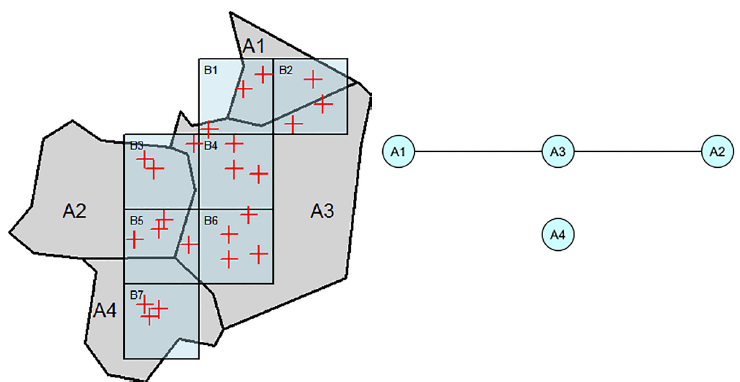
\includegraphics[width=0.9\linewidth]{figures/Differencing_issues/to_graph.png}
\caption{Overlapping areas and the corresponding graph; source: \citet{Costemalle_2019}.}
%\vspace{0.15 cm}
\raggedright \textit{\footnotesize Reading note: The graph on the right shows the links between the municipalities. The municipality $A1$ is linked to $A3$ because the tile $B1$ crosses both municipalities and has a population in each of them ($2$ in $A1$ and $1$ in $A3$).}
\label{fig:graph_ex}
\end{figure}

First, a graph is built by linking areas: two areas are connected, if a tile has its population spread across both of them. Figure~\ref{fig:graph_ex} shows an overlapping case and its corresponding graph. Area $A4$ is not connected to the others, since no tile is populated at once in $A4$ and another area. This first step builds some independent connected sub-graphs that can be handled separately.

As the first step can generate very large sub-graphs, \cite{Costemalle_2019} introduces several ways of reducing each of them, including merging nodes (zones) if the population of tiles that connect them is above the threshold in each zone (see Fig.~\ref{fig:merge_nodes}). Next, each sub-graph is split in smaller components according to the complementarity of internal and external differences. Finally, these differences are applied to all the sub-graphs to detect differencing issues (i.e. overlapped areas with population below a given threshold).


\begin{figure}[H]
\centering
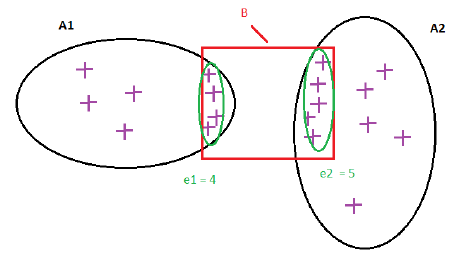
\includegraphics[width=0.7\linewidth]{figures/Differencing_issues/merge_nodes.png}
\caption{Merging nodes}
\vspace{0.15 cm}
\textit{\footnotesize Reading note: As the connecting tile has a population above the threshold in $A1$ ($e1=4$) and in $A2$ ($e2=5$), the two areas will be merged together in the graph.}
\label{fig:merge_nodes}
\end{figure}

In practice, the user of the package \texttt{diffman} \citep{diffman} only needs to call the \texttt{find\_pbm\_diff()} function to detect the differencing issues between two sets of non-nested areas.

\subsection{How to prevent geographical differencing issues}

Once detected, how can differencing problems be prevented? 

\cite{BuronFontaine2018} list four possibilities:

\begin{itemize}
    \item If areas can be modified, redraw their borders so as to eliminate the overlaps;
    \item if areas can't be redrawn, merge some of them so as to eliminate the overlaps;
    \item suppress some data;
    \item perturb some data.
\end{itemize}

\subsubsection{Suppressive approach}

With a suppressive method (see section \ref{sec:aux_suppr}), the suppression of the overlapping zone is inefficient. Actually, to prevent both internal and external differencing, one has to suppress one tile in the internal region and one tile in the external region.

In Figure~\ref{fig:prevent}, in order to avoid differencing the two tiles in blue have to be suppressed. The left one prevents the internal differencing and the right one prevents the external differencing.

\begin{figure}[ht]
\centering
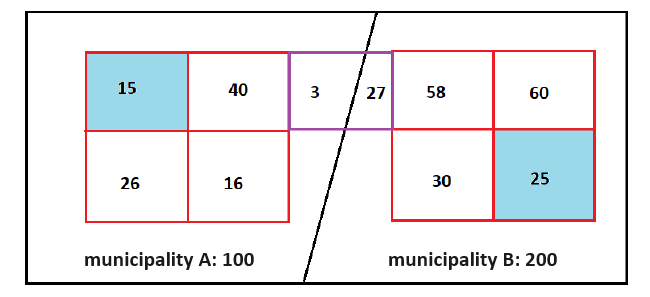
\includegraphics[width=0.8\linewidth]{figures/Differencing_issues/prevent_2_en.png}
\caption{Suppression pattern against differencing.}
\vspace{0.15 cm}
\textit{\footnotesize Reading note: The blue tiles are the suppressed tiles, preventing differencing.}
\label{fig:prevent}
\end{figure}

It is quite difficult to prevent geographical differencing issues with a suppressive approach in some real cases, such as census releases. Indeed, if many geographical sets of areas are released at the same time, the differencing potential has to be checked for every combination of overlapping sets. Nevertheless, if nested areas are used, it is sufficient to check and fix differencing issues with the smallest areas and the overlapping ones.

\subsubsection{Perturbative approach}

A perturbative approach can tackle the problem efficiently and systematically if and only if the method injects noise in \emph{every} cell, like the Cell Key Method (section \ref{sec:ckm}) or any rounding or noise injection method. A swapping method (section \ref{sec:trs}), for example, doesn't tackle the problem on its own.
